% !TEX spellcheck = en_US



% ~~~~~~~~~~~~~~~~~~~~~~~~~~~~~~~~~~~~~~~ V
% (NC) 2024Haluk Bingol
% github.com/halukbingol/LaTeX-Templates
%
% Licensees may copy, distribute, display, and perform the work and make derivative works 
% and remixes based on it only for non-commercial purposes. 
% ~~~~~~~~~~~~~~~~~~~~~~~~~~~~~~~~~~~~~~~ A




%\documentclass{beamer}
\documentclass[10pt]{beamer}
	\usetheme{Dresden}
%	\usetheme{Copenhagen}
%	\usetheme{Marburg}
%	\usetheme{CambridgeUS}
%	\usetheme{Warsaw}
%	\usetheme{AnnArbor}

%	\usecolortheme{orchid}
	
%	\usecolortheme{}
%	\useinnertheme{}
%	\useoutertheme{}
%	\setbeamertemplate{bibliography item}[text]
\usepackage{beamerthemesplit}
%\usecolortheme{default}
%\usecolortheme{structure}
%\usepackage{beamerthemesplit} // Activate for custom appearance

\useoutertheme{split}
\useinnertheme{rounded} 
\usecolortheme{whale}
\usecolortheme{orchid}
\setbeamertemplate{blocks}[rounded]




% ~~~~~~~~~~~~~~~~~~~~~~~~~~~~~~~~~~~~~~~ V HB lib
\usepackage{../hbcommon/hbdatastructures} 
\usepackage{../hbcommon/hbpresentation} 
% ~~~~~~~~~~~~~~~~~~~~~~~~~~~~~~~~~~~~~~~ A HB lib




% ~~~~~~~~~~~~~~~~~~~~~~~~~~~~~~~~~~~~~~~ V specific	
\usepackage[normalem]{ulem} %strikethroug

\usepackage{tikz-qtree} % tree
\usepackage{adjustbox} % tikzpicture alignment

%\usepackage{moreverb} % tab control
\usepackage{fancyvrb} % tab

% https://tex.stackexchange.com/questions/118173/how-to-write-ceil-and-floor-in-latex
\usepackage{mathtools}
\DeclarePairedDelimiter\ceil{\lceil}{\rceil}
\DeclarePairedDelimiter\floor{\lfloor}{\rfloor}

%\newcommand{\hDummy}{dummy}
% ~~~~~~~~~~~~~~~~~~~~~~~~~~~~~~~~~~~~~~~ A specific	






% ~~~~~~~~~~~~~~~~~~~~~~~~~~~~~~~~~~~~~~~ V
\title{
	cis112\\
	Tree
}

\author[Bingol]{Haluk O. Bingol}

\institute{
	Faculty of Computer and Information Sciences\\
	Yeditepe University
}

%\date{
%	cis112\\ 
%	Yeditepe University, 2024-02-25
%}
\date{
	{\tiny \hbTimeStamp}
}
% ~~~~~~~~~~~~~~~~~~~~~~~~~~~~~~~~~~~~~~~ A



\begin{document}
% ~~~~~~~~~~~~~~~~~~~~~~~~~~~~~~~~~~~~~~~ 




% ~~~~~~~~~~~~~~~~~~~~~~~~~~~~~~~~~~~~~~~ V Title
\frame{\titlepage}
% ~~~~~~~~~~~~~~~~~~~~~~~~~~~~~~~~~~~~~~~ A 




% ~~~~~~~~~~~~~~~~~~~~~~~~~~~~~~~~~~~~~~~ V Content
\begin{frame}[t]\frametitle{Content}
	\begin{columns}[T]
	\begin{column}{.5\linewidth}   
	    	\tableofcontents[hideallsubsections]
		
		\hCite{ %
	\cite{knuth1973artv1}, %
	\cite{cormen2022introduction}, %
	\cite{preiss1999}, %
	\cite{aho1974design}, %
	\cite{horowitz1982fundamentals}, %
	\cite{horstmann2016big}, %
	\cite{grimaldi2006discrete}
}
	\end{column}
	\begin{column}{.5\linewidth}
		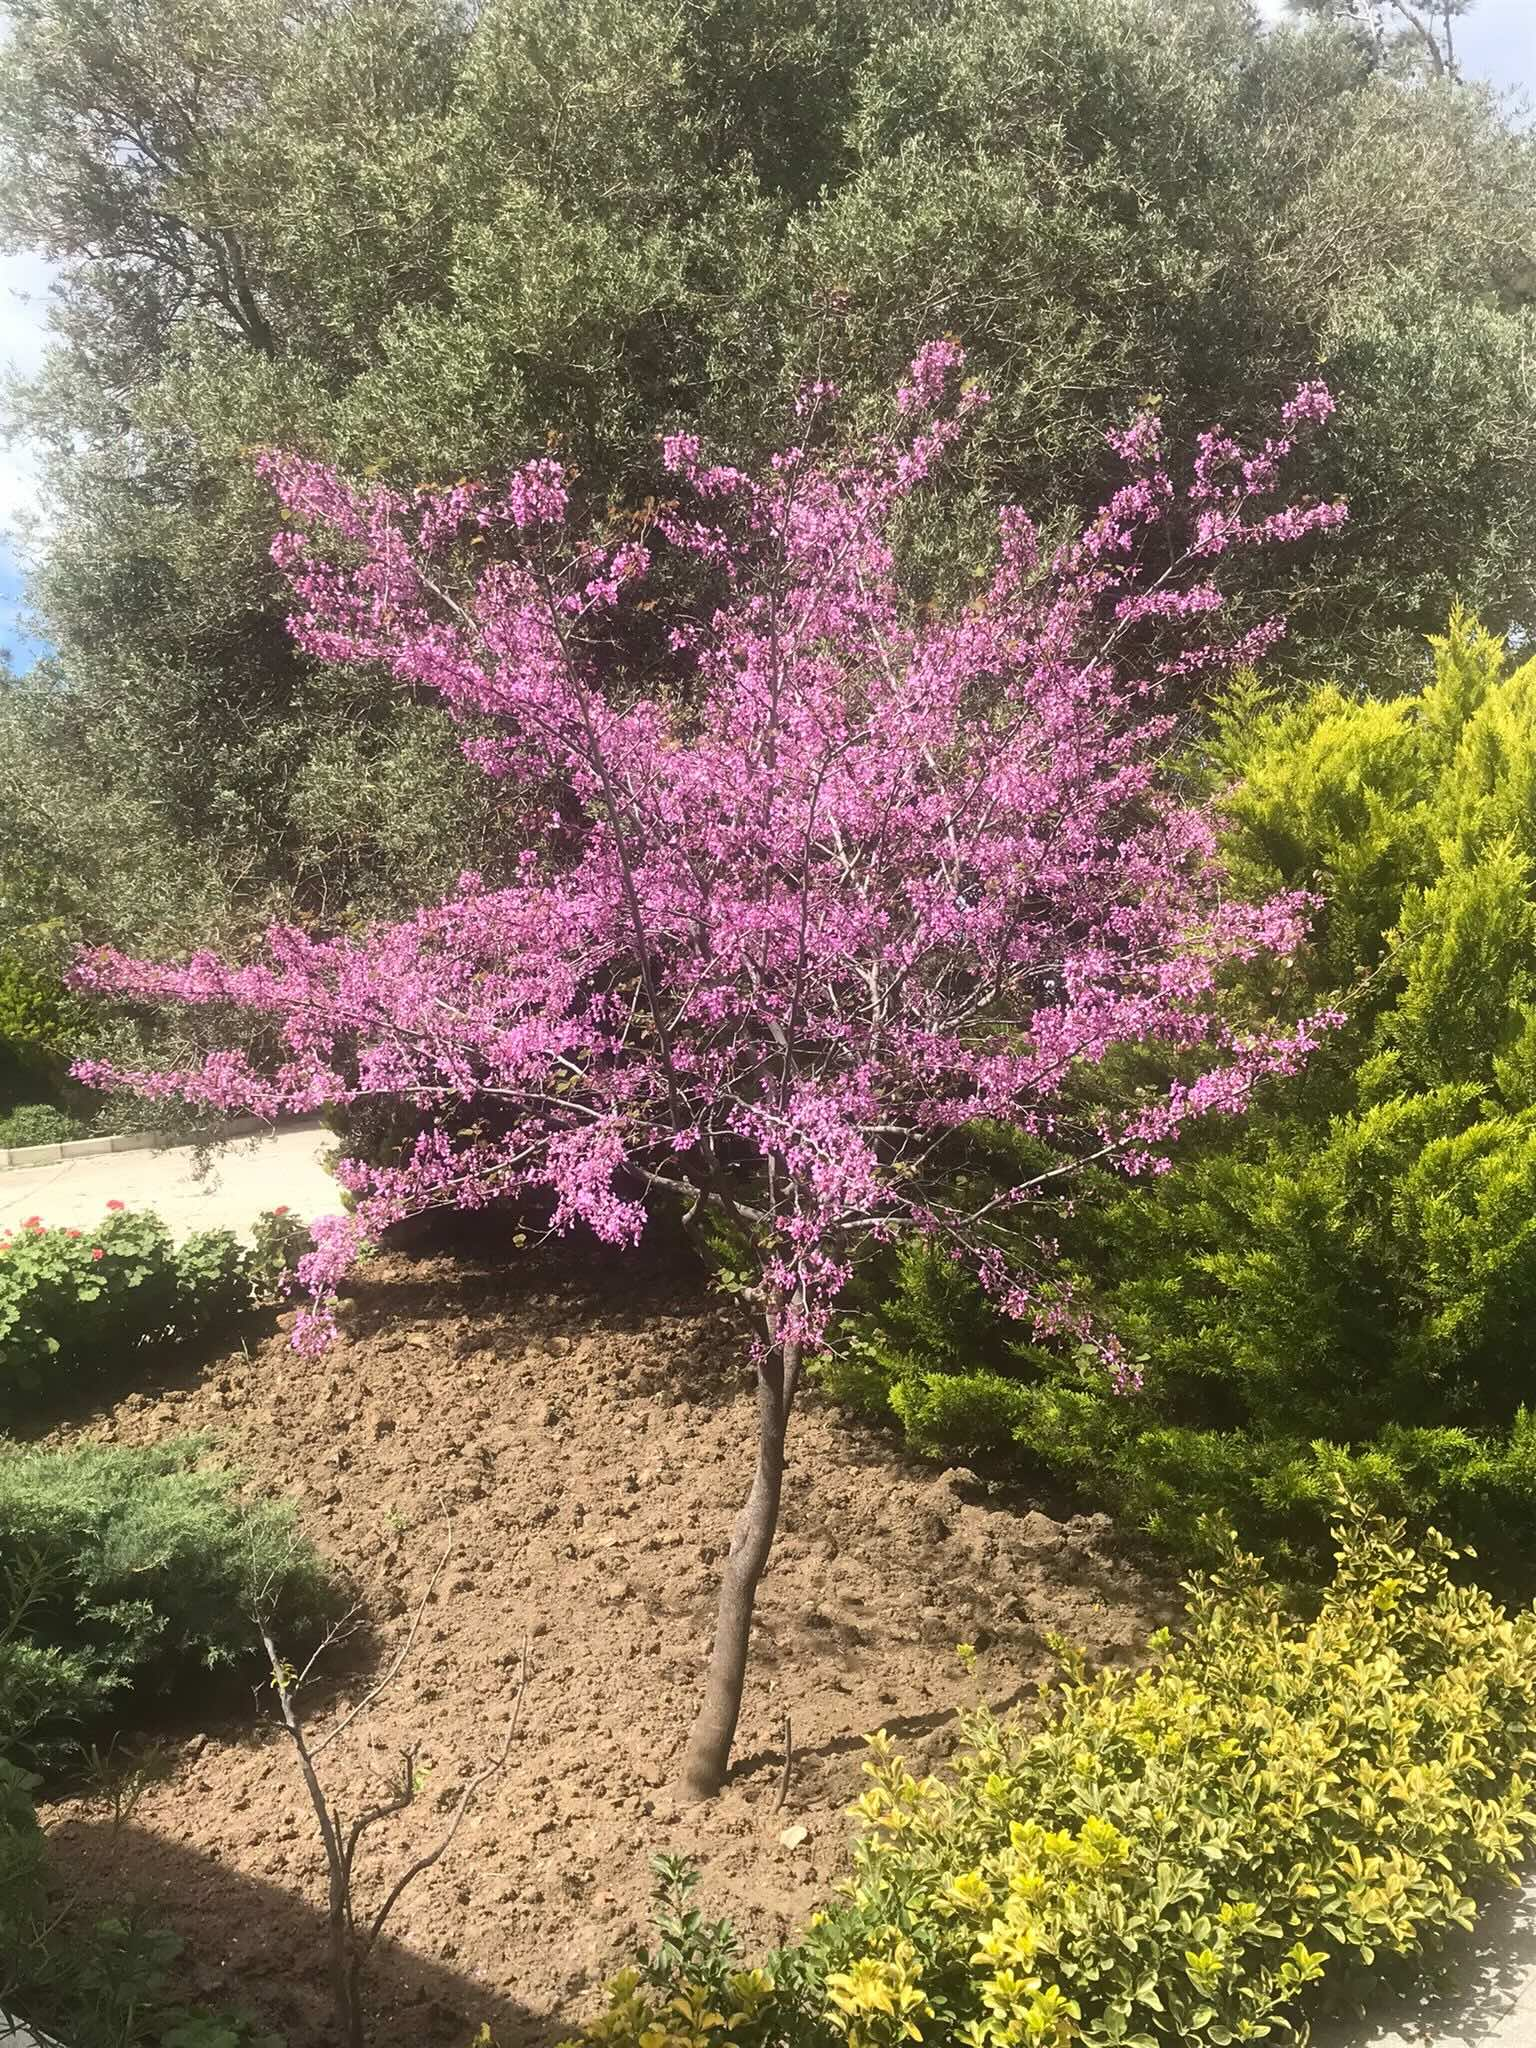
\includegraphics[width=.8\columnwidth]
		{fig/fig-Erguvan.jpg}
%		{example-image}
	\end{column}
	\end{columns}
\end{frame}
% ~~~~~~~~~~~~~~~~~~~~~~~~~~~~~~~~~~~~~~~ A




% ~~~~~~~~~~~~~~~~~~~~~~~~~~~~~~~~~~~~~~ V
\hSection{Motivation}{Hierarchy}{}
% ~~~~~~~~~~~~~~~~~~~~~~~~~~~~~~~~~~~~~~ A




\subsection{Some hierarchies}
%\subsection{Directory hierarchy}
% ~~~~~~~~~~~~~~~~~~~~~~~~~~~~~~~~~~~~~~ V
\begin{frame}[t,fragile] \frametitle{Directory hierarchy}
%\begin{frame}[t]\frametitle{aaa}
	\begin{columns}[T] % >>>>
	\begin{column}{.7\linewidth} % ++++ V
{\footnotesize 	
\begin{Verbatim}[tabsize=4]
MyDisk (D)
|- Private (E)
|  |- Family (F)
|- School (G)
|  |- CIS111 (H)
|  |  |- Project-1 (I)
|  |- CIS112 (J)
|  |  |- Project-1 (K)
|  |  |- Project-2 (L)
|  |- CIS114 (M)
\end{Verbatim}
} % fsize
	\end{column} % ++++ A
	\begin{column}{.3\linewidth} % ++++ V
		\begin{tikzpicture}
	\tikzset{every leaf node/.style={font=\sffamily}}
	\Tree
	[.$D$
		[.$E$
			[.$F$ ]
		]
		[.$G$
			[.$H$ 
				[.$I$ ]
			]
			[.$J$ 
				[.$K$ ]
				[.$L$ ]
			]
			[.$M$  ]
		]
	]
\end{tikzpicture}

	\end{column} % ++++ A
	\end{columns} % <<<<
\end{frame}
% ~~~~~~~~~~~~~~~~~~~~~~~~~~~~~~~~~~~~~~ A



%\subsection{Organizational hierarchy}
% ~~~~~~~~~~~~~~~~~~~~~~~~~~~~~~~~~~~~~~ V
\begin{frame}[t,fragile] \frametitle{Organizational hierarchy}
%\begin{frame}[t]\frametitle{aaa}
	\begin{columns}[T] % >>>>
	\begin{column}{.7\linewidth} % ++++ V
{\footnotesize 	
\begin{Verbatim}[tabsize=4]
General Manager {
	VP {
		Production {
		}
	}
	VP {
		Human Resources {
			class I {
			}
		}
		Finance {
			Accounting {}
			Treasury  {}
		}
		Sales {}
	}
}
\end{Verbatim}
} % fsize
	\end{column} % ++++ A
	\begin{column}{.3\linewidth} % ++++ V
		\begin{tikzpicture}
	\tikzset{every leaf node/.style={font=\sffamily}}
	\Tree
	[.$D$
		[.$E$
			[.$F$ ]
		]
		[.$G$
			[.$H$ 
				[.$I$ ]
			]
			[.$J$ 
				[.$K$ ]
				[.$L$ ]
			]
			[.$M$  ]
		]
	]
\end{tikzpicture}

	\end{column} % ++++ A
	\end{columns} % <<<<
\end{frame}
% ~~~~~~~~~~~~~~~~~~~~~~~~~~~~~~~~~~~~~~ A




%\subsection{Subset hierarchy}
% ~~~~~~~~~~~~~~~~~~~~~~~~~~~~~~~~~~~~~~ V
\begin{frame}[t,fragile] \frametitle{Subset hierarchy}
%\begin{frame}[t]\frametitle{aaa}
	\begin{columns}[T] % >>>>
	\begin{column}{.7\linewidth} % ++++ V
		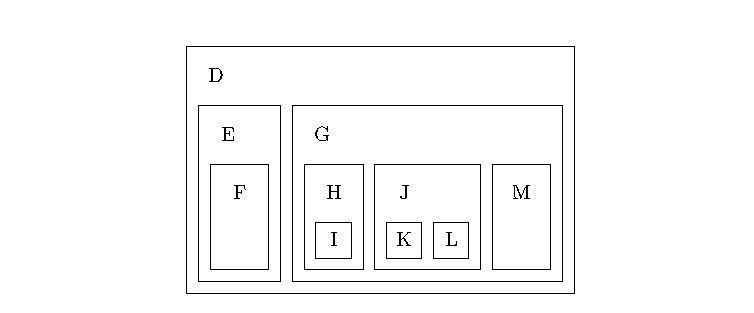
\includegraphics[width=.8\columnwidth]
			{fig/fig-setHierarchy}
		\\
		\hCite{ %
			\cite{knuth1973artv1}, %
			\cite{preiss1999}%
		}
			
	\end{column} % ++++ A
	\begin{column}{.3\linewidth} % ++++ V
		\begin{tikzpicture}
	\tikzset{every leaf node/.style={font=\sffamily}}
	\Tree
	[.$D$
		[.$E$
			[.$F$ ]
		]
		[.$G$
			[.$H$ 
				[.$I$ ]
			]
			[.$J$ 
				[.$K$ ]
				[.$L$ ]
			]
			[.$M$  ]
		]
	]
\end{tikzpicture}

	\end{column} % ++++ A
	\end{columns} % <<<<
\end{frame}
% ~~~~~~~~~~~~~~~~~~~~~~~~~~~~~~~~~~~~~~ A





%\subsection{Inner class hierarchy}
% ~~~~~~~~~~~~~~~~~~~~~~~~~~~~~~~~~~~~~~ V
\begin{frame}[t,fragile] \frametitle{Inner class hierarchy}
%\begin{frame}[t]\frametitle{aaa}
	\begin{columns}[T] % >>>>
	\begin{column}{.7\linewidth} % ++++ V
{\footnotesize 	
\begin{Verbatim}[tabsize=4]
class D {
	class E {
		class F {
		}
	}
	class G {
		class H {
			class I {
			}
		}
		class J {
			class K {}
			class L {}
		}
		class M {}
	}
}
\end{Verbatim}
}
	\end{column} % ++++ A
	\begin{column}{.3\linewidth} % ++++ V
		\begin{tikzpicture}
	\tikzset{every leaf node/.style={font=\sffamily}}
	\Tree
	[.$D$
		[.$E$
			[.$F$ ]
		]
		[.$G$
			[.$H$ 
				[.$I$ ]
			]
			[.$J$ 
				[.$K$ ]
				[.$L$ ]
			]
			[.$M$  ]
		]
	]
\end{tikzpicture}

	\end{column} % ++++ A
	\end{columns} % <<<<
\end{frame}
% ~~~~~~~~~~~~~~~~~~~~~~~~~~~~~~~~~~~~~~ A




\subsection{Expressions}
% ~~~~~~~~~~~~~~~~~~~~~~~~~~~~~~~~~~~~~~ V
\begin{frame}[t,fragile] \frametitle{Expressions}
%\begin{frame}[t]\frametitle{aaa}
	\begin{columns}[T] % >>>>
	\begin{column}{.7\linewidth} % ++++ V
		\[
			(-F) + ( (-I) \times (K + L) \times M)
		\]
		{\center
		\begin{tikzpicture}
			\tikzset{every leaf node/.style={font=\sffamily}}
			\Tree
			[.$+$
				[.$-$
					[.$6$ ]
				]
				[.$*$
					[.$-$ 
						[.$4$ ]
					]
					[.$+$ 
						[.$3$ ]
						[.$5$ ]
					]
					[.$7$  ]
				]
			]
		\end{tikzpicture}\\
		
		\[(-6) + (-4) \times (3 + 5) \times 7\]
		} % center
	
	\end{column} % ++++ A
	\begin{column}{.3\linewidth} % ++++ V
		\begin{tikzpicture}
	\tikzset{every leaf node/.style={font=\sffamily}}
	\Tree
	[.$D$
		[.$E$
			[.$F$ ]
		]
		[.$G$
			[.$H$ 
				[.$I$ ]
			]
			[.$J$ 
				[.$K$ ]
				[.$L$ ]
			]
			[.$M$  ]
		]
	]
\end{tikzpicture}

	\end{column} % ++++ A
	\end{columns} % <<<<
\end{frame}
% ~~~~~~~~~~~~~~~~~~~~~~~~~~~~~~~~~~~~~~ A




\subsection{Linguistics}
% ~~~~~~~~~~~~~~~~~~~~~~~~~~~~~~~~~~~~~~ V
\begin{frame}[t,fragile] \frametitle{Linguistics}
%\begin{frame}[t]\frametitle{aaa}
	\begin{columns}[T] % >>>>
	\begin{column}{.5\linewidth} % ++++ V
		``the cat sat on the mat.''\\
		
		\vspace{1cm}
		
		
		S: Sentence\\
		N: Noun\\
		V: Verb\\
		A: Article\\
		NP: Noun Phrase\\
		PP: Prepositional Phrase\\
		VP: Verb Phrase\\
		
		
		
	\end{column} % ++++ A
	\begin{column}{.5\linewidth} % ++++ V
	{\small 
		\begin{tikzpicture}
%	\tikzset{every leaf node/.style={font=\sffamily}}
	\tikzset{frontier/.style={distance from root=150pt}}
	\Tree 
	[.S 
		[.NP 
			[.A \hEmph{the} ] 
			[.N \hEmph{cat} ] ]
		[.VP 
			[.V \hEmph{sat} ]
			[.PP
				[.P \hEmph{on} ]
				[.NP 
					[.A \hEmph{the} ]
					[.N \hEmph{mat} ]
				]
			] 
		] 
	]
\end{tikzpicture}

	}
	\end{column} % ++++ A
	\end{columns} % <<<<
\end{frame}
% ~~~~~~~~~~~~~~~~~~~~~~~~~~~~~~~~~~~~~~ A




% ~~~~~~~~~~~~~~~~~~~~~~~~~~~~~~~~~~~~~~ V
\begin{frame}[t,fragile] \frametitle{Linguistics}
%\begin{frame}[t]\frametitle{aaa}
	\begin{columns}[T] % >>>>
	\begin{column}{.5\linewidth} % ++++ V
		``the girl hit the ball with a bat.''\\
		
		\vspace{1cm}
		
		S: Sentence\\
		N: Noun\\
		V: Verb\\
		A: Article\\
		NP: Noun Phrase\\
		PP: Prepositional Phrase\\
		VP: Verb Phrase\\
		
		
		
	\end{column} % ++++ A
	\begin{column}{.5\linewidth} % ++++ V
	{\small 
		\begin{tikzpicture}
%	\tikzset{every leaf node/.style={font=\sffamily}}
	\tikzset{frontier/.style={distance from root=150pt}}
	\Tree 
	[.S 
		[.NP 
			[.A \hEmph{the} ] 
			[.N \hEmph{girl} ]
		]
		[.VP 
			[.V \hEmph{hit} ]
			[.NP 
				[.A \hEmph{the} ] 
				[.N \hEmph{ball} ]
			]
			[.PP
				[.P \hEmph{with} ]
				[.NP 
					[.A \hEmph{a} ]
					[.N \hEmph{bat} ]
				]
			] 
		] 
	]
\end{tikzpicture}

	}
	\end{column} % ++++ A
	\end{columns} % <<<<
\end{frame}
% ~~~~~~~~~~~~~~~~~~~~~~~~~~~~~~~~~~~~~~ A




% ~~~~~~~~~~~~~~~~~~~~~~~~~~~~~~~~~~~~~~ V
\hSection{Definitions}{}{\hCite{ %
	\cite{knuth1973artv1}, %
	\cite{cormen2022introduction}, %
	\cite{preiss1999}, %
	\cite{aho1974design}, %
	\cite{horowitz1982fundamentals}, %
	\cite{horstmann2016big}, %
	\cite{grimaldi2006discrete}
}}
% ~~~~~~~~~~~~~~~~~~~~~~~~~~~~~~~~~~~~~~ A



\subsection{Tree and Subtree}
% ~~~~~~~~~~~~~~~~~~~~~~~~~~~~~~~~~~~~~~ V
\begin{frame}[t]\frametitle{Tree and Subtree}

	\vspace{-0.5cm}
	\begin{columns}[T] % >>>>
	\begin{column}{.6\linewidth} % ++++ V
	{\footnotesize 
		\begin{definition}[Mathematical]
			A \hDefined{tree \(T\)}  is a finite, non-empty set of \hDefined{node}s
			\[T = \{ r \} \cup T_1 \cup T_2 \cup \cdots \cup T_n,\]
			with the following properties:
			\begin{enumerate}
			
				\item 
				A designated node of the set, \hEmph{$r$},
				is called the \hDefined{root} of the tree; and
				
				\item 
				The remaining nodes are partitioned into $n\ge0$ subsets,
				$T_1$, $T_2$, \ldots, $T_n$,
				each of which is a tree. $T_{i}$ is called a \hDefined{subtree}.
			\end{enumerate}			
		\end{definition}
		
		\textbf{Q.}
		What is the minimum number of vertices in a tree?
		
		\textbf{Notation.}
		\begin{itemize}
			
			\item 
			\hEmph{$T=\{r,T_1,T_2,\ldots,T_n\}$} denotes the tree $T$.				

			\item
			\hEmph{$V$} is the set of \hEmph{vertices} (nodes) in $T$.
			
			\item
			$\hEmph{v}\in V$ is a \hEmph{vertex} (node) of $T$.
		\end{itemize}
	} %fsize
	\end{column} % ++++ A
	\begin{column}{.4\linewidth} % ++++ V
		\begin{example}
		{\scriptsize
			\begin{tabular}{c c c}
	\adjustbox{valign=t}{			
		\begin{tikzpicture}
			\tikzset{every leaf node/.style={font=\sffamily}}
			\Tree
			[.{A} ]
		\end{tikzpicture}
	} % \adjustbox
	&
	\adjustbox{valign=t}{	
		\begin{tikzpicture}
			\tikzset{every leaf node/.style={font=\sffamily}}
			\Tree
			[.{B} 
				[.{C} ]
			]
		\end{tikzpicture}
	} % \adjustbox
	&
	\adjustbox{valign=t}{	
		\begin{tikzpicture}
			\tikzset{every leaf node/.style={font=\sffamily}}
			\Tree
			[.{0}
				[.$1$
					[.$3$  ]
					[.$4$  ]
					[.$5$  ]
				]
				[.$2$
					[.$6$ ]
					[.$7$ 
						[.$8$ ]
						[.$9$ ]
					]
				]
			]
		\end{tikzpicture}
	} % \adjustbox
\end{tabular}

			\\		
			$A$ is a tree with 1 node.\\
			$B$ is a tree with 2 nodes.\\
			$0$ is a tree with 9 nodes.\\
			$1$ is a tree with 4 nodes.\\
			$2$ is a tree with 5 nodes.\\
			$4$ is a tree with 1 node.\\		
		} %\scriptsize
		\end{example}

	\end{column} % ++++ A
	\end{columns} % <<<<
\end{frame}
% ~~~~~~~~~~~~~~~~~~~~~~~~~~~~~~~~~~~~~~ A



\subsection{Degree, Leaf, Parent, Child and Siblings}
% ~~~~~~~~~~~~~~~~~~~~~~~~~~~~~~~~~~~~~~ V
\begin{frame}[t]\frametitle{Degree and Leaf}
	\begin{columns}[T] % >>>>
	\begin{column}{.6\linewidth} % ++++ V
	{\footnotesize 
		\begin{definition}
			Let $T = \{r, T_{1}, T_{2}, \ldots, T_{n}\}$ be a tree.\\					    
			The \hDefined{degree} of a node is the number of subtrees associated with that node.				
		\end{definition}	
		\begin{example}
			{\scriptsize
			The degree of $r$ in tree $T = \{r, T_{1}, T_{2}, \ldots, T_{n}\}$  is $n$.
			} %fsize
		\end{example}		
		\begin{definition}
			A node of degree 0  is called a \hDefined{leaf}.
		\end{definition}	
		\textbf{Q.}
		Is it possible to have a negative degree?		
	} %fsize
	\end{column} % ++++ A
	\begin{column}{.4\linewidth} % ++++ V
		\begin{example}
		{\scriptsize
			\begin{tabular}{c c c}
	\adjustbox{valign=t}{			
		\begin{tikzpicture}
			\tikzset{every leaf node/.style={font=\sffamily}}
			\Tree
			[.{A} ]
		\end{tikzpicture}
	} % \adjustbox
	&
	\adjustbox{valign=t}{	
		\begin{tikzpicture}
			\tikzset{every leaf node/.style={font=\sffamily}}
			\Tree
			[.{B} 
				[.{C} ]
			]
		\end{tikzpicture}
	} % \adjustbox
	&
	\adjustbox{valign=t}{	
		\begin{tikzpicture}
			\tikzset{every leaf node/.style={font=\sffamily}}
			\Tree
			[.{0}
				[.$1$
					[.$3$  ]
					[.$4$  ]
					[.$5$  ]
				]
				[.$2$
					[.$6$ ]
					[.$7$ 
						[.$8$ ]
						[.$9$ ]
					]
				]
			]
		\end{tikzpicture}
	} % \adjustbox
\end{tabular}

			\\
			Nodes $A$, $C$, $3$ are leafs.\\
			Degree of node $B$ is 1.\\
			Degree of node $0$ is 2.\\
			Degree of node $1$ is 3.\\
		} %\scriptsize
		\end{example}
	\end{column} % ++++ A
	\end{columns} % <<<<
\end{frame}
% ~~~~~~~~~~~~~~~~~~~~~~~~~~~~~~~~~~~~~~ A



%\subsection{Parent, Child and Siblings}
% ~~~~~~~~~~~~~~~~~~~~~~~~~~~~~~~~~~~~~~ V
\begin{frame}[t]\frametitle{Parent, Child and Siblings}
	\begin{columns}[T] % >>>>
	\begin{column}{.6\linewidth} % ++++ V
	{\footnotesize 
		\begin{definition}
			Let $T = \{r, T_{1}, T_{2}, \ldots, T_{n}\}$, $n \ge 0$ be a tree $T$.					    
			Let  $r_{i}$ be the root of subtree  $T_{i}$ .
			Then 
			\begin{itemize}
				
				\item
				 $r$ is called the \hDefined{parent} of $r_{i}$ .
	
				\item 
				$r_{i}$ is called a \hDefined{child} of $r$
				 
				 \item
				 Roots $r_{i}$ and $r_{j}$ of distinct subtrees $T_{i}$ 
				 and $T_{j}$ of tree $T$ are called \hDefined{siblings}.
			\end{itemize}
		\end{definition}	
		\textbf{Q.}
		What is the minimum and maximum number of 
		\begin{itemize}
			
			\item 
			parents of a node $a$?
			
			\item 
			children of a node $a$?
			
			\item 
			siblings of a node $a$?
			
		\end{itemize}
	} %fsize
	\end{column} % ++++ A
	\begin{column}{.4\linewidth} % ++++ V
		\begin{example}
		{\scriptsize
			\begin{tabular}{c c c}
	\adjustbox{valign=t}{			
		\begin{tikzpicture}
			\tikzset{every leaf node/.style={font=\sffamily}}
			\Tree
			[.{A} ]
		\end{tikzpicture}
	} % \adjustbox
	&
	\adjustbox{valign=t}{	
		\begin{tikzpicture}
			\tikzset{every leaf node/.style={font=\sffamily}}
			\Tree
			[.{B} 
				[.{C} ]
			]
		\end{tikzpicture}
	} % \adjustbox
	&
	\adjustbox{valign=t}{	
		\begin{tikzpicture}
			\tikzset{every leaf node/.style={font=\sffamily}}
			\Tree
			[.{0}
				[.$1$
					[.$3$  ]
					[.$4$  ]
					[.$5$  ]
				]
				[.$2$
					[.$6$ ]
					[.$7$ 
						[.$8$ ]
						[.$9$ ]
					]
				]
			]
		\end{tikzpicture}
	} % \adjustbox
\end{tabular}

			\\
			Node $B$ is parent of node $C$.\\
			Node $C$ is a child of node $B$.\\
			Nodes $3$ and $4$ are siblings.\\
		} %\scriptsize
		\end{example}
	\end{column} % ++++ A
	\end{columns} % <<<<
\end{frame}
% ~~~~~~~~~~~~~~~~~~~~~~~~~~~~~~~~~~~~~~ A



\subsection{Path and Path Length}
% ~~~~~~~~~~~~~~~~~~~~~~~~~~~~~~~~~~~~~~ V
\begin{frame}[t]\frametitle{Path and Path Length}
	\begin{columns}[T] % >>>>
	\begin{column}{.6\linewidth} % ++++ V
	{\footnotesize 
		\begin{definition}
			Let $T = \{ r, T_{1}, T_{2}, \ldots, T_{n} \}$ be a tree $T$.					    
			Let  $V$ be the set of nodes in  $T$.

			\begin{itemize}
				
				\item 
				A \hDefined{path} is a non-empty sequence of nodes 
				$P = ( v_{1}, v_{2}, \dotsc, v_{k} )$
				where,  $v_{i} \in V$ for $1 \le i \le k$,
				such that $v_{i}$ is parent of $v_{i + 1}$.
				
				\item 
				The \hDefined{length} of path $P$ is $k - 1$.
				
			\end{itemize}
		\end{definition}	
		
		\textbf{Remark.}
		\begin{itemize}
			
			\item 
			Direction of a path is from root to leaf.
			
			\item 
			There is a \hEmph{unique} path from root to any node in the tree.			
		\end{itemize}
		
		\textbf{Q.}
		Is $(v)$ a path?
	} %fsize
	\end{column} % ++++ A
	\begin{column}{.4\linewidth} % ++++ V
		\begin{example}
		{\scriptsize
%			\begin{tabular}{c c c}
	\adjustbox{valign=t}{			
		\begin{tikzpicture}
			\tikzset{every leaf node/.style={font=\sffamily}}
			\Tree
			[.{A} ]
		\end{tikzpicture}
	} % \adjustbox
	&
	\adjustbox{valign=t}{	
		\begin{tikzpicture}
			\tikzset{every leaf node/.style={font=\sffamily}}
			\Tree
			[.{B} 
				[.{C} ]
			]
		\end{tikzpicture}
	} % \adjustbox
	&
	\adjustbox{valign=t}{	
		\begin{tikzpicture}
			\tikzset{every leaf node/.style={font=\sffamily}}
			\Tree
			[.{0}
				[.$1$
					[.$3$  ]
					[.$4$  ]
					[.$5$  ]
				]
				[.$2$
					[.$6$ ]
					[.$7$ 
						[.$8$ ]
						[.$9$ ]
					]
				]
			]
		\end{tikzpicture}
	} % \adjustbox
\end{tabular}

			\begin{tikzpicture}
	\tikzset{every leaf node/.style={font=\sffamily}}
	\Tree
	[.{0}
		[.$1$
			[.$3$  ]
			[.$4$  ]
			[.$5$  ]
		]
		[.$2$
			[.$6$ ]
			[.$7$ 
				[.$8$ ]
				[.$9$ ]
			]
		]
	]
\end{tikzpicture}

			\\
			$(2, 7, 9)$ is a path.\\
			$(0,1)$ is a path.\\
			Unique path to node $8$ is the path $(0, 2, 7, 8)$\\
		} %\scriptsize
		\end{example}
	\end{column} % ++++ A
	\end{columns} % <<<<
\end{frame}
% ~~~~~~~~~~~~~~~~~~~~~~~~~~~~~~~~~~~~~~ A



\subsection{Ancestor and Desendant}
% ~~~~~~~~~~~~~~~~~~~~~~~~~~~~~~~~~~~~~~ V
\begin{frame}[t]\frametitle{Ancestor and Descendant}
	\begin{columns}[T] % >>>>
	\begin{column}{.6\linewidth} % ++++ V
	{\footnotesize 
		\begin{definition}
			Let $T$  be a tree with the set of nodes $V$.
			Suppose there exists a path $P$ from $v_{i}$ to $v_{j}$ for  $v_{i}, v_{j} \in V$,
			Then
			\begin{itemize}
				\item
				the vertex $v_{i}$ is an  \hDefined{ancestor} of $v_{j}$;

				\item
				the vertex $v_{j}$ is a  \hDefined{descendant} of $v_{i}$.
			\end{itemize}
			
			If the length of $P$ is non-zero, then
			\begin{itemize}
				\item
				the vertex $v_{i}$ is a  \hDefined{proper ancestor} of $v_{j}$;

				\item
				the vertex $v_{j}$ is a  \hDefined{proper descendant} of $v_{i}$.
			\end{itemize}
		\end{definition}	

		\textbf{Remark.}
		\begin{itemize}
			
			\item 
			A path is from ancestor to descendant.
			
			\item 
			Vertex $v$ is ancestor of itself.\\
			
			\item 
			Vertex $v$ is descendant of itself.\\
		
		\end{itemize}
	} %fsize
	\end{column} % ++++ A
	\begin{column}{.4\linewidth} % ++++ V
		\begin{example}
		{\scriptsize
			\begin{tikzpicture}
	\tikzset{every leaf node/.style={font=\sffamily}}
	\Tree
	[.{0}
		[.$1$
			[.$3$  ]
			[.$4$  ]
			[.$5$  ]
		]
		[.$2$
			[.$6$ ]
			[.$7$ 
				[.$8$ ]
				[.$9$ ]
			]
		]
	]
\end{tikzpicture}

			\\
			$2$ is ancestor of $7$.\\
			$9$ is descendant of $2$.\\
		} % fsize
		\end{example}
	\end{column} % ++++ A
	\end{columns} % <<<<
\end{frame}
% ~~~~~~~~~~~~~~~~~~~~~~~~~~~~~~~~~~~~~~ A



\subsection{Level and Height}
% ~~~~~~~~~~~~~~~~~~~~~~~~~~~~~~~~~~~~~~ V
\begin{frame}[t]\frametitle{Level (Depth) and Height}
	\begin{columns}[T] % >>>>
	\begin{column}{.6\linewidth} % ++++ V
	{\footnotesize 
		\begin{definition}
			Let $T$  be a tree with the set of nodes $V$.
			\begin{itemize}
				\item
				The \hDefined{level} (\hDefined{depth}) of a node $v \in V$
				in a tree $T$ is the length of the unique path in $T$
				from its root $r$ to the node $v$.
		
				\item
				The \hDefined{height} of a node $v\in V$ in a tree $T$
				is the length of the longest path from node $v$ to a leaf.
			
				\item
				The \hDefined{height} of a tree $T$ is the height of its root $r$.
			\end{itemize}
		\end{definition}	

		\textbf{Remark.}
		\begin{itemize}
			
			\item 
			The root $r$ of $T$ is at level-0.
			
			\item
			The roots of the subtrees of $r$ are at level-1.
			
			\item
			The leaves are at height 0.
		
		\end{itemize}
	} %fsize
	\end{column} % ++++ A
	\begin{column}{.4\linewidth} % ++++ V
		\begin{example}
		{\scriptsize
			\begin{tikzpicture}
	\tikzset{every leaf node/.style={font=\sffamily}}
	\Tree
	[.{0}
		[.$1$
			[.$3$  ]
			[.$4$  ]
			[.$5$  ]
		]
		[.$2$
			[.$6$ ]
			[.$7$ 
				[.$8$ ]
				[.$9$ ]
			]
		]
	]
\end{tikzpicture}

			\\
			Node $0$ is at level-0.\\
			Node $1$ is at level-1.\\
			Node $4$ is at level-2.\\
			Node $9$ is at level-3.\\
			Height of node $7$ is 1.\\
			Height of node $2$ is 2.\\
			Height of node $0$ is 3.\\
			Height of \hEmph{tree} $T$ is 3.\\
		} %\scriptsize
		\end{example}
	\end{column} % ++++ A
	\end{columns} % <<<<
\end{frame}
% ~~~~~~~~~~~~~~~~~~~~~~~~~~~~~~~~~~~~~~ A




% ~~~~~~~~~~~~~~~~~~~~~~~~~~~~~~~~~~~~~~ V
\hSection{Tree as a Data Structure}{}{}
% ~~~~~~~~~~~~~~~~~~~~~~~~~~~~~~~~~~~~~~ A




\subsection{$N$-ary Trees}
% ~~~~~~~~~~~~~~~~~~~~~~~~~~~~~~~~~~~~~~ V
\begin{frame}[t]\frametitle{$N$-ary Trees}
	\begin{columns}[T] % >>>>
	\begin{column}{.5\linewidth} % ++++ V
		{\small
 		\begin{definition}[Data Structure]
		An \hDefined{$N$-ary tree} $T$ is a finite set of nodes
		with the following properties:
		\begin{enumerate}
			\item 
			Either the set is empty, $T=\emptyset$; or
			
			\item 
			The set consists of a \hEmph{root}, \hEmph{$r$},
			and exactly $N$ distinct $N$-ary trees, \hEmph{$T_{i}$}.
			
			I.e., the remaining nodes are partitioned into $N \ge 0$ subsets,
			$T_{0}$, $T_{1}$, \ldots, $T_{N-1}$, each of which is an $N$-ary tree
			such that $T = \{ r, T_{0}, T_{1}, \ldots, T_{N-1} \}$.
		\end{enumerate}
		\end{definition}
		} % fsize
	\end{column} % ++++ A
	\begin{column}{.5\linewidth} % ++++ V
		{\small 
		\textbf{Note that}
		\begin{itemize}
	
			\item
			The \hEmph{degree} of each node of an $N$-ary tree is either zero or $N$

			\item
			The \hDefined{empty tree}, $T = \emptyset$, is a tree.
			That is, 
			it is an object of the same type as a non-empty tree

		\end{itemize}
		} % fsize
	\end{column} % ++++ A
	\end{columns} % <<<<
\end{frame}
% ~~~~~~~~~~~~~~~~~~~~~~~~~~~~~~~~~~~~~~ A




\subsection{Binary Trees}
% ~~~~~~~~~~~~~~~~~~~~~~~~~~~~~~~~~~~~~~ V
\begin{frame}[t]\frametitle{Binary Trees}
	\begin{columns}[T] % >>>>
	\begin{column}{.5\linewidth} % ++++ V
		{\small
		\begin{definition}[Data Structure]
		A \hDefined{binary tree} $T$
		is a finite set of \hDefined{nodes}
		with the following properties:
		\begin{enumerate}
		
			\item 
			Either the set is empty, $T=\emptyset$; or
			
			\item 
			The set consists of a \hDefined{root}, \hEmph{$r$},
			and exactly two distinct binary trees \hEmph{$T_{L}$} and \hEmph{$T_{R}$},
			$T = \{ r, T_{L}, T_{R} \}$.
		\end{enumerate}
		The tree $T_{L}$ is called the \hDefined{left subtree} of $T$,
		and the tree $T_{R}$ is called the \hDefined{right subtree} of $T$.
		\end{definition}
		} % fsize
	\end{column} % ++++ A
	\begin{column}{.5\linewidth} % ++++ V
		{\small 
		\textbf{Note that}
		\begin{itemize}
	
			\item
			The \hEmph{degree} of each node of an binary tree is either 0, 1  or 2.

			\item
			A binary tree of height $h \ge 0$ has at most $2^{h+1}-1$ nodes
			
			\item
			Therefore the height of a binary tree with $n$  nodes is at least 
			$\lceil \log_{2} n+1 \rceil - 1$.

		\end{itemize}
		} % fsize
	\end{column} % ++++ A
	\end{columns} % <<<<
\end{frame}
% ~~~~~~~~~~~~~~~~~~~~~~~~~~~~~~~~~~~~~~ A




\subsection{Ordered Trees}
% ~~~~~~~~~~~~~~~~~~~~~~~~~~~~~~~~~~~~~~ V
\begin{frame}[t]\frametitle{Ordered Trees}
	\begin{columns}[T] % >>>>
	\begin{column}{.5\linewidth} % ++++ V
		{\small
 		\begin{definition}
		An \hDefined{ordered tree} is a tree in which the order of the subtrees matters.
 		\end{definition}
		} % fsize
		
		\textbf{Warning.}
		Unless stated otherwise, all trees we deal with are ordered trees.
	\end{column} % ++++ A
	\begin{column}{.5\linewidth} % ++++ V
		{\small
		\begin{example}
			Tree $T_{12} = \{ r, T_{1}, T_{2} \}$ is different than
			tree $T_{21} = \{ r, T_{2}, T_{1} \}$.
			
			{\tiny 			
				\begin{tikzpicture}
	\tikzset{every leaf node/.style={font=\sffamily}}
	\Tree
	[.{\hEmph{$root_{T}$} }
		[.\hEmph{$root_{T_{1}}$}   \edge[roof]; {subtree-$T_{1}$} ]
		[.\hEmph{$root_{T_{2}}$}   \edge[roof]; {subtree-$T_{2}$} ]
	]
\end{tikzpicture}

				\quad
				\begin{tikzpicture}
	\tikzset{every leaf node/.style={font=\sffamily}}
	\Tree
	[.{\hEmph{$root_{T}$} }
		[.\hEmph{$root_{T_{2}}$}   \edge[roof]; {subtree-$T_{2}$} ]
		[.\hEmph{$root_{T_{1}}$}   \edge[roof]; {subtree-$T_{1}$} ]
	]
\end{tikzpicture}

				} % fsize
			\end{example}
		} % fsize
	\end{column} % ++++ A
	\end{columns} % <<<<
\end{frame}
% ~~~~~~~~~~~~~~~~~~~~~~~~~~~~~~~~~~~~~~ A




% ~~~~~~~~~~~~~~~~~~~~~~~~~~~~~~~~~~~~~~ V
\hSection{Balanced Trees}{}{}
% ~~~~~~~~~~~~~~~~~~~~~~~~~~~~~~~~~~~~~~ A



\subsection{Balanced Trees}
% ~~~~~~~~~~~~~~~~~~~~~~~~~~~~~~~~~~~~~~ V
\begin{frame}[t]\frametitle{Balanced Trees}
	\begin{columns}[T] % >>>>
	\begin{column}{.5\linewidth} % ++++ V
		\begin{definition}
			 A tree $T = \{ r, T_{1}, T_{2}, \ldots, T_{n} \}$ is \hDefined{balanced} 
			 iff
			\begin{itemize}
			
				\item
				$T$ is empty or
			
				\item
				$T_{1}, T_{2}, \ldots, T_{n}$ have ``almost the same height''.
			\end{itemize}		 
		\end{definition}
		
		\textbf{Remark.}
		\begin{itemize}
			
			\item 
			Consider ``almost the same height'' as difference of 1.

			\item			
			How to \hEmph{keep a tree balanced} is an important issue that 
			we will deal with

		\end{itemize}
		
	\end{column} % ++++ A
	\begin{column}{.5\linewidth} % ++++ V
		\begin{example}
		{\scriptsize
			\begin{tabular}{c c}
			balanced
			& unbalanced
			\\
			\begin{tikzpicture}
	\tikzset{every leaf node/.style={font=\sffamily}}
	\Tree
	[.$1$
		[.$2$
			[.$4$ 
				[.$8$ ]
				[.$9$ ]
			]
			[.$5$
				[.$10$ ]
				[.$11$ ]				
			]
		]
		[.$3$
			[.$6$ ]
			[.$7$ ]
		]
	]
\end{tikzpicture}

			&\begin{tikzpicture}
	\tikzset{every leaf node/.style={font=\sffamily}}
	\Tree
	[.$1$
		[.$2$
			[.~ ]
			[.$5$
				[.$10$ ]
				[.$11$ ]				
			]
		]
		[.$3$ ]
	]
\end{tikzpicture}

			\\
			\end{tabular}
		} %\scriptsize
		\end{example}
	\end{column} % ++++ A
	\end{columns} % <<<<
\end{frame}
% ~~~~~~~~~~~~~~~~~~~~~~~~~~~~~~~~~~~~~~ A



\subsection{Complete Binary Tree}
% ~~~~~~~~~~~~~~~~~~~~~~~~~~~~~~~~~~~~~~ V
\begin{frame}[t]\frametitle{Complete Binary Tree}
	\begin{columns}[T] % >>>>
	\begin{column}{.5\linewidth} % ++++ V
		\begin{definition}
			 A binary tree $T = \{ r, T_{L}, T_{R} \}$ is called \hDefined{complete binary tree}
			 iff
			 each node has either 0 or 2 degrees.
		\end{definition}
	\end{column} % ++++ A
	\begin{column}{.5\linewidth} % ++++ V
		\begin{example}
		{\scriptsize
			\begin{tabular}{c c}
			complete binary tree
			&
			not
			\\
			\begin{tikzpicture}
	\tikzset{every leaf node/.style={font=\sffamily}}
	\Tree
	[.$1$
		[.$2$
			[.$4$ 
				[.$8$ ]
				[.$9$ ]
			]
			[.$5$
				[.$10$ ]
				[.$11$ ]				
			]
		]
		[.$3$
			[.$6$ ]
			[.$7$ ]
		]
	]
\end{tikzpicture}

			&\begin{tikzpicture}
	\tikzset{every leaf node/.style={font=\sffamily}}
	\Tree
	[.$1$
		[.$2$
			[.~ ]
			[.$5$
				[.$10$ ]
				[.$11$ ]				
			]
		]
		[.$3$ ]
	]
\end{tikzpicture}

			\\
			~
			&
			due to node 2.
			\end{tabular}
		} %\scriptsize
		\end{example}
	\end{column} % ++++ A
	\end{columns} % <<<<
\end{frame}
% ~~~~~~~~~~~~~~~~~~~~~~~~~~~~~~~~~~~~~~ A







\subsection{Full Binary Tree}
% ~~~~~~~~~~~~~~~~~~~~~~~~~~~~~~~~~~~~~~ V
\begin{frame}[t]\frametitle{Full Binary Tree}
	\begin{columns}[T] % >>>>
	\begin{column}{.5\linewidth} % ++++ V
		\begin{definition}
			 A binary tree $T$ is called \hDefined{full binary tree}
			 iff
			 all the leafs in $T$ are at level $h$.
		\hCite{%
			\cite{grimaldi2006discrete}%
		}
		\end{definition}
		
		\textbf{Remark.}
		\begin{itemize}
			
			\item 
			Some books, 
			such as
			\hCite{%
				\cite{cormen2022introduction}%
			},
			calls it \emph{complete binary tree}.

			\item
			A full binary tree is a special form with the property that 
			\hEmph{maximum possible number of nodes in a minimum possible height}.
		\end{itemize}
		
		
	\end{column} % ++++ A
	\begin{column}{.5\linewidth} % ++++ V
		{\scriptsize
		\begin{example}
			\begin{tikzpicture}
	\tikzset{every leaf node/.style={font=\sffamily}}
	\Tree
	[.$1$
		[.$2$
			[.$4$ 
				[.$8$ ]
				[.$9$ ]
			]
			[.$5$
				[.$10$ ]
				[.$11$ ]				
			]
		]
		[.$3$
			[.$6$
				[.$12$ ]
				[.$13$ ]
			]
			[.$7$ 
				[.$14$ ]
				[.$15$ ]
			]
		]
	]
\end{tikzpicture}

		\end{example}
		} %\scriptsize
	\end{column} % ++++ A
	\end{columns} % <<<<
\end{frame}
% ~~~~~~~~~~~~~~~~~~~~~~~~~~~~~~~~~~~~~~ A




\subsection{Relations in Number of Nodes and Height}
% ~~~~~~~~~~~~~~~~~~~~~~~~~~~~~~~~~~~~~~ V
\begin{frame}[t]\frametitle{Relations in Number of Nodes and Height}
	\begin{columns}[T] % >>>>
	\begin{column}{.5\linewidth} % ++++ V
		{\footnotesize
 	    	In a full binary tree
		\begin{itemize}
			
			\item
			at \hEmph{level-0}, there is only $2^{0} = 1$ node: 1
			
			\item
			at \hEmph{level-1}, there are $2^{1} = 2$ nodes: 2, 3
			
			\item
			at \hEmph{level-2},  there are $2^{2} = 4$ nodes: 4, 5, 6, 7
						
			\item
			at \hEmph{level-3},  there are $2^{3} = 8$ nodes: 8, 9, 10, 11, 12, 13, 14, 15
			
		\end{itemize}
		\textbf{Generalization.}
		\begin{itemize}
						
			\item
			In a \hEmph{full binary tree}
			\begin{itemize}
				
				\item
				at level-\hEmph{$\ell$},  there are $2^{\ell}$nodes.
				
				\item 
				height \hEmph{$h$} $\implies$ $n = 2^{h +1} - 1$.
				
				\item
				number of nodes \hEmph{$n$} $\implies$ 
				$h = \log_{2}(n + 1) - 1$.
				
			\end{itemize}
			
			\item 
			In any \hEmph{binary tree}, $n \le 2^{h +1} - 1$.
		
		\end{itemize}
		} % fsize

		
	\end{column} % ++++ A
	\begin{column}{.5\linewidth} % ++++ V
		\begin{example}
		{\scriptsize
			\begin{tikzpicture}
	\tikzset{every leaf node/.style={font=\sffamily}}
	\Tree
	[.$1$
		[.$2$
			[.$4$ 
				[.$8$ ]
				[.$9$ ]
			]
			[.$5$
				[.$10$ ]
				[.$11$ ]				
			]
		]
		[.$3$
			[.$6$
				[.$12$ ]
				[.$13$ ]
			]
			[.$7$ 
				[.$14$ ]
				[.$15$ ]
			]
		]
	]
\end{tikzpicture}

			\\
			A full binary tree.
			Levels: 0, 1, 2, and 3.
			The number of nodes: $n = 15$ and
			height: $h = 3$.
			\\
			Then
			\hEmph{$n = 2^{h +1} - 1$} and
			\hEmph{$h = \log_{2}(n + 1)$}.
			
		} %\scriptsize
		\end{example}
		
		{\footnotesize  
		\textbf{Theorem.} $ (1 + x^{1} + \dotsc + x^{n})(x-1) = x^{n + 1} -1$
		} % fsize
	\end{column} % ++++ A
	\end{columns} % <<<<
\end{frame}
% ~~~~~~~~~~~~~~~~~~~~~~~~~~~~~~~~~~~~~~ A




% ~~~~~~~~~~~~~~~~~~~~~~~~~~~~~~~~~~~~~~ V
\begin{frame}[t]\frametitle{Relations in Number of Nodes and Height}
{\footnotesize
	\begin{columns}[T] % >>>>
	\begin{column}{.5\linewidth} % ++++ V
	    	Height of a tree is very important
		\begin{itemize}
			\item
			In \hEmph{search}, number of steps is \hEmph{directly related to the height}
			
			\item
			The relation between $n$ and $h$ is \hEmph{logarithmic},
			i.e., $h = \ceil*{\log_{2}(n + 1) - 1}$.
			It is due to nonlinearity of tree data structure
			
			\item
			Therefore, searching in trees is \hEmph{$O(\log n)$} rather than $O(n)$,
			which is a big improvement for big $n$ values.
			
			\item 
			Because of these nice properties, 
			trees are very frequently used in CS.
			
		\end{itemize}
	\end{column} % ++++ A
	\begin{column}{.5\linewidth} % ++++ V
		{\footnotesize
 	    	In any \hEmph{binary tree},
		\begin{itemize}
				
			\item 
			Given $h$, 
			\hEmph{$n \le 2^{h +1} - 1$}
			
			\item
			 Given $n$,
			 \hEmph{ $h \ge \ceil*{\log_{2}(n + 1) - 1}$}
		
		\end{itemize}
		} % fsize

		\begin{center}
%		$n \le 2^{h +1} - 1$ and $h \ge \ceil*{\log_{2}(n + 1) - 1}$
		\begin{tabular}{| r | r | r |}
			\hline
			$n$ &$\log_{2}(n + 1) - 1$ &$h$\\
			\hline
			1,000 &8.97 &9\\
			1,000,000 &18.93 &19\\
			10,000,000 &22.25 &23\\
			100,000,000 &25.58 &26\\
			1,000,000,000 &28.90 &29\\
			\hline
		\end{tabular}
		\end{center}
		
		
	\end{column} % ++++ A
	\end{columns} % <<<<
} % fsize
\end{frame}
% ~~~~~~~~~~~~~~~~~~~~~~~~~~~~~~~~~~~~~~ A




% ~~~~~~~~~~~~~~~~~~~~~~~~~~~~~~~~~~~~~~ V
\hSection{Implementation}{}{}
% ~~~~~~~~~~~~~~~~~~~~~~~~~~~~~~~~~~~~~~ A
%
%
%
%% ~~~~~~~~~~~~~~~~~~~~~~~~~~~~~~~~~~~~~~ V
%\hSection{Abstraction}{}{}
%% ~~~~~~~~~~~~~~~~~~~~~~~~~~~~~~~~~~~~~~ A




% ~~~~~~~~~~~~~~~~~~~~~~~~~~~~~~~~~~~~~~ V
\begin{frame}[t]\frametitle{Tree}
	\begin{columns}[T] % >>>>
	\begin{column}{.5\linewidth} % ++++ V
		{\footnotesize 
	    	Tree $T$ is a data structure 
		\begin{itemize}
			\item
			with a \hEmph{$T.root$} pointing to the \hEmph{root} node of the tree
			
			\item
			 $T.root.parent = \mathsf{NIL}$
			
			\item
			Let $x$ be a node of $T$
			
			\begin{itemize}
				
				\item
				If $x.parent = \mathsf{NIL}$,\\
				then $x$ is the $root$,\\
				i.e., \hEmph{root} is the only node with parent is NIL
				
				\item 
				If $x.subtree_{i} = \mathsf{NIL}$,\\
				then $x$ has no subtree $T_{i}$ \\
				i.e., the subtree $T_{i}$ is empty
				
			\end{itemize}
			
		\end{itemize}
		
		\hCite{ %
	\cite{knuth1973artv1}, %
	\cite{cormen2022introduction}, %
	\cite{preiss1999}, %
	\cite{aho1974design}, %
	\cite{horowitz1982fundamentals}, %
	\cite{horstmann2016big}, %
	\cite{grimaldi2006discrete}
}
		} % fsize

	\end{column} % ++++ A
	\begin{column}{.5\linewidth} % ++++ V
{\footnotesize 
		\begin{tikzpicture}
	\tikzset{every leaf node/.style={font=\sffamily}}
	\Tree
	[.\texttt{T.root}
		[.{\hEmph{root} } \edge[roof]; {RestOfTheTree}
		]
	]
\end{tikzpicture}

		\begin{tikzpicture}
	\tikzset{every leaf node/.style={font=\sffamily}}
	\Tree
	[.\texttt{T.root}
		[.{\hEmph{$root_{T}$} }
			[.\hEmph{$root_{T_{1}}$}   \edge[roof]; {subtree-$T_{1}$} ]
			[.\hEmph{$root_{T_{2}}$}   \edge[roof]; {subtree-$T_{2}$} ]
			[.\hEmph{$\dotsc$}  \edge[roof]; {$\dotsc$} ]
			[.\hEmph{$root_{T_{N}}$} \edge[roof]; {subtree-$T_{N}$} ]
		]
	]
\end{tikzpicture}

} %fsize

	\end{column} % ++++ A
	\end{columns} % <<<<
\end{frame}
% ~~~~~~~~~~~~~~~~~~~~~~~~~~~~~~~~~~~~~~ A




\subsection{Node of N-ary Tree}
% ~~~~~~~~~~~~~~~~~~~~~~~~~~~~~~~~~~~~~~ V
\begin{frame}[t]\frametitle{N-ary Tree}
	\vspace{-0.3cm}
	\begin{columns}[T] % >>>>
	\begin{column}{.5\linewidth} % ++++ V		
		{\tiny 
		\begin{algorithm}[H]
			\SetKwData{Data}{\texttt{data}}
			\SetKwData{P}{\texttt{parent}}
			\Begin{
				\Data\\
				\P	\tcp*[f]{{\tiny reference to the parent}}\\
				child1	\tcp*[f]{{\tiny reference to the first subtree}}\\
				child2	\tcp*[f]{{\tiny reference to the second subtree}}\\
				...\\
				childN	\tcp*[f]{{\tiny reference to the $N$'th subtree}}\\
			    
				\caption{{\footnotesize Node for $N$-ary tree: General case}}
			}
		\end{algorithm}
		} % \tiny

	\textbf{Remark.}
	In the most general case of a tree,
	each node may have different number $N$ of subtrees.
	
	This is a problem.

	\end{column} % ++++ A
	\begin{column}{.5\linewidth} % ++++ V
%		\includegraphics[width=\columnwidth]
%			{fig/fig-TreeN-ary}
		\centering
		{\tiny
		\begin{tikzpicture}
			\tikzset{every leaf node/.style={font=\sffamily}}
			\Tree
			[.{parent}
				[.{\textbf{node}} 
					[.{subtree-1} ]
					[.{subtree-2} ]
					[.{...} ]
					[.{subtree-N} ]
				]
			]
		\end{tikzpicture}
		} % fsize
		\phantom{line} \\
		\phantom{line} \\
		\phantom{line} \\
		{\tiny
		\begin{tikzpicture}
			\tikzset{every leaf node/.style={font=\sffamily}}
			\Tree
			[.{a} 
				[.{b} 
					[.{e} ]
					[.{f} ]
					[.{g} ]
					[.{h} ]
				]
				[.{c} ]
				[.{...} ]
				[.{d} 
					[.{i} ]
					[.{j} ]
					[.{h} ]
				]
			]
		\end{tikzpicture}
		} % fsize

	\end{column} % ++++ A
	\end{columns} % <<<<
\end{frame}
% ~~~~~~~~~~~~~~~~~~~~~~~~~~~~~~~~~~~~~~ A




% ~~~~~~~~~~~~~~~~~~~~~~~~~~~~~~~~~~~~~~ V
\begin{frame}[t]\frametitle{$N$-ary Trees: Left-child, right-sibling representation}
	\vspace{-0.3cm}
	\begin{columns}[T] % >>>>
	\begin{column}{.5\linewidth} % ++++ V		
		{\tiny 
		\begin{algorithm}[H]
			\SetKwData{Data}{\texttt{data}}
			\SetKwData{P}{\texttt{parent}}
			\Begin{
				\Data\\
				\P	\tcp*[f]{{\tiny reference to the parent}}\\
				leftChild	\tcp*[f]{{\tiny reference to the left child}}\\
				rightSibling	\tcp*[f]{{\tiny reference to the right sibling}}\\
			    
				\caption{{\footnotesize Node for Left-child, right-sibling}}
			}
		\end{algorithm}
		} % \tiny

	    	Use node with three pointers:
		\begin{itemize}
		
			\item
			\hEmph{parent}: points the parent
		
			\item
			\hEmph{leftChild}: points the left child
		
			\item
			\hEmph{rightSibling}: points the right sibling
			
		\end{itemize}

		\textbf{Remark.}
		Now node becomes uniform,
		i.e., independent of degree.

	\end{column} % ++++ A
	\begin{column}{.5\linewidth} % ++++ V
		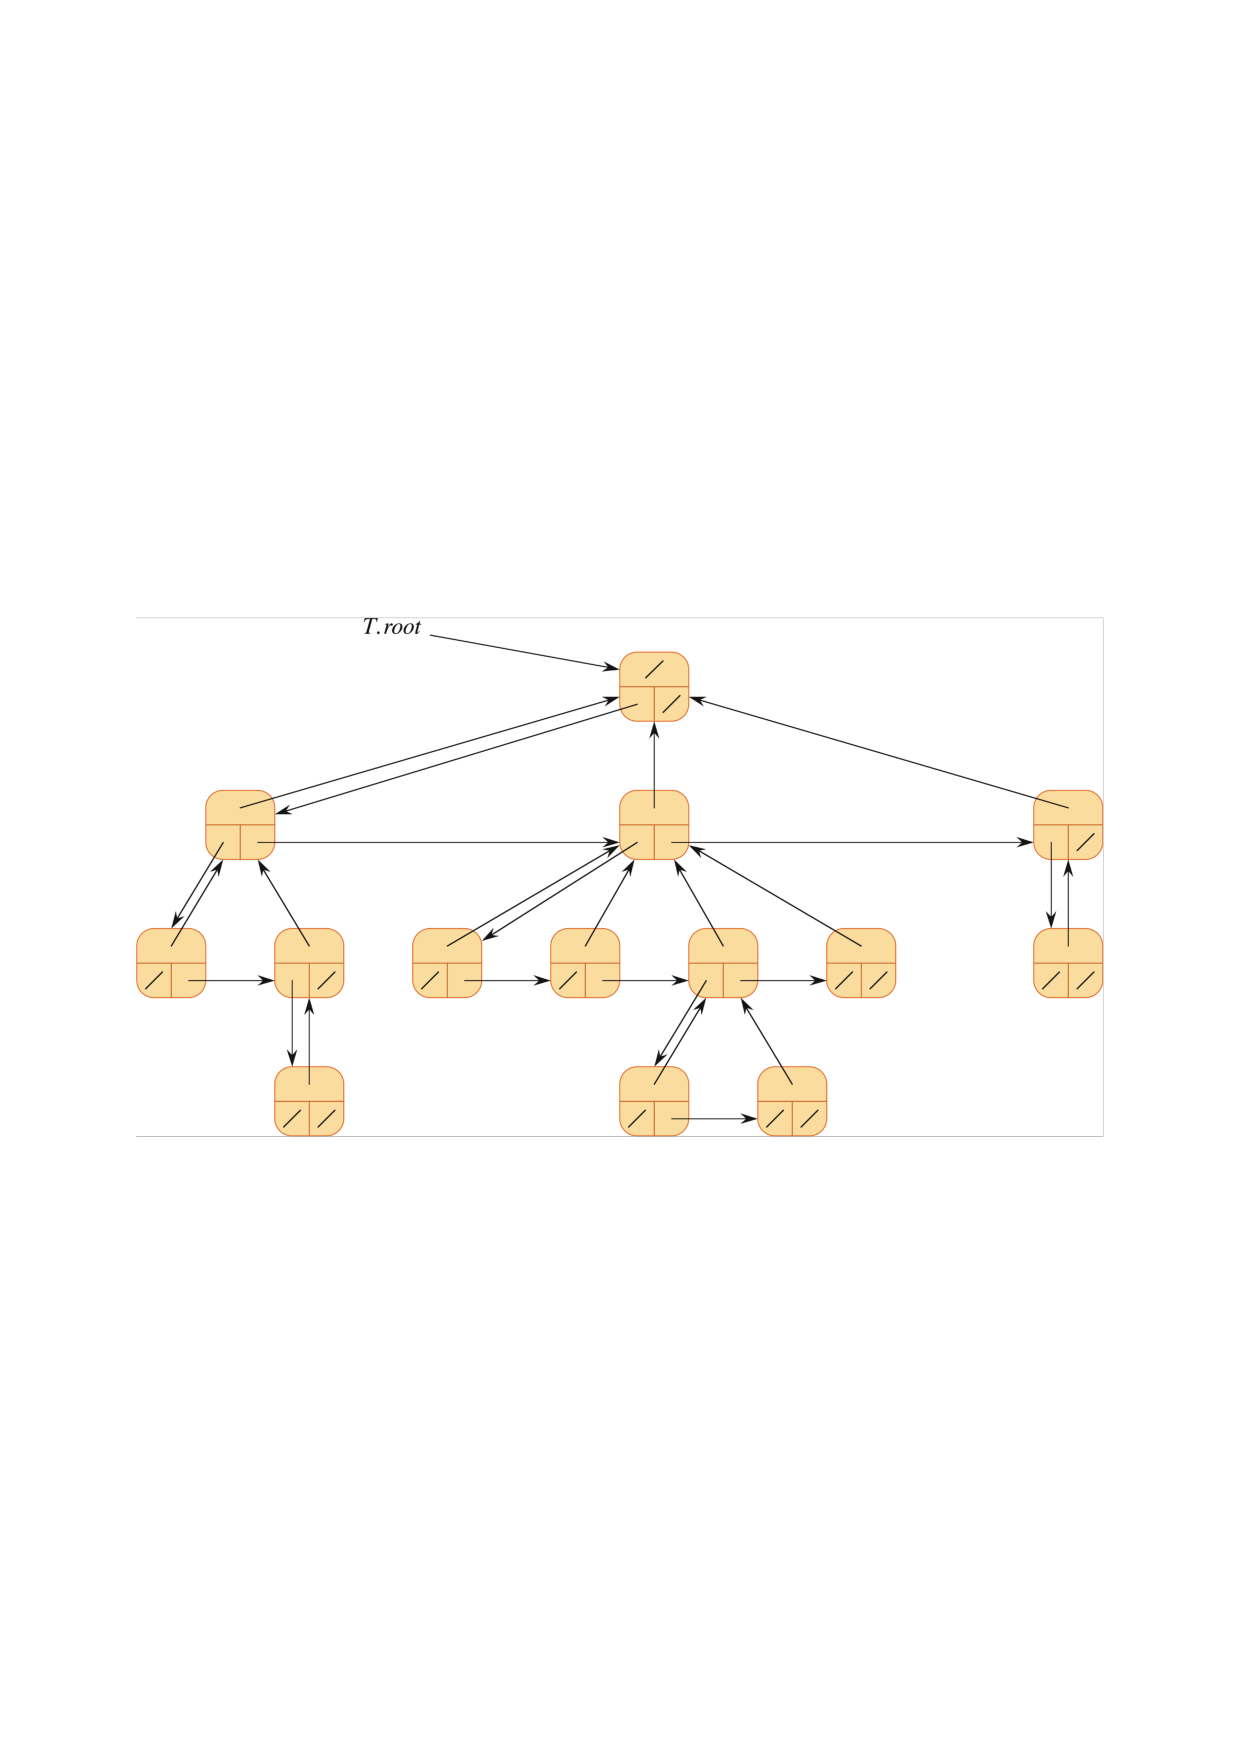
\includegraphics[width=\columnwidth]
			{fig/fig-TreeN-ary}
		{\tiny
		\begin{tikzpicture}
			\tikzset{every leaf node/.style={font=\sffamily}}
			\Tree
			[.{parent}
				[.{\textbf{node}} 
					[.{leftChild} ]
					[.{rightSibling} ]
				]
			]
		\end{tikzpicture}
		} % fsize

	\end{column} % ++++ A
	\end{columns} % <<<<
\end{frame}
% ~~~~~~~~~~~~~~~~~~~~~~~~~~~~~~~~~~~~~~ A



\subsection{Binary Tree}
% ~~~~~~~~~~~~~~~~~~~~~~~~~~~~~~~~~~~~~~ V
\begin{frame}[t]\frametitle{Binary Tree}
	\vspace{-0.3cm}
	\begin{columns}[T] % >>>>
	\begin{column}{.5\linewidth} % ++++ V
		{\tiny 
		\begin{algorithm}[H]
			\SetKwData{Data}{\texttt{data}}
			\SetKwData{P}{\texttt{parent}}
			\SetKwData{L}{\texttt{left}}
			\SetKwData{R}{\texttt{right}}
			\Begin{
				\Data\\
				\P	\tcp*[f]{{\tiny reference to the parent}}\\
				\L	\tcp*[f]{{\tiny reference to the left child}}\\
				\R	\tcp*[f]{{\tiny reference to the right child}}\\
			    
				\caption{{\footnotesize Node for binary tree}}
			}
		\end{algorithm}
		} % \tiny

		{\footnotesize
			In \hEmph{binary tree}, 
			each node has 0, 1 or 2 subtrees.
		
%				\hEmph{Binary tree representation}
				
				Use node with three pointers:
				\begin{itemize}
				
					\item
					\hEmph{parent}: points the parent
				
					\item
					\hEmph{left}: points the left child
				
					\item
					\hEmph{right}: points the right child
					
				\end{itemize}
		} % fsize

		
	\end{column} % ++++ A
	\begin{column}{.5\linewidth} % ++++ V
		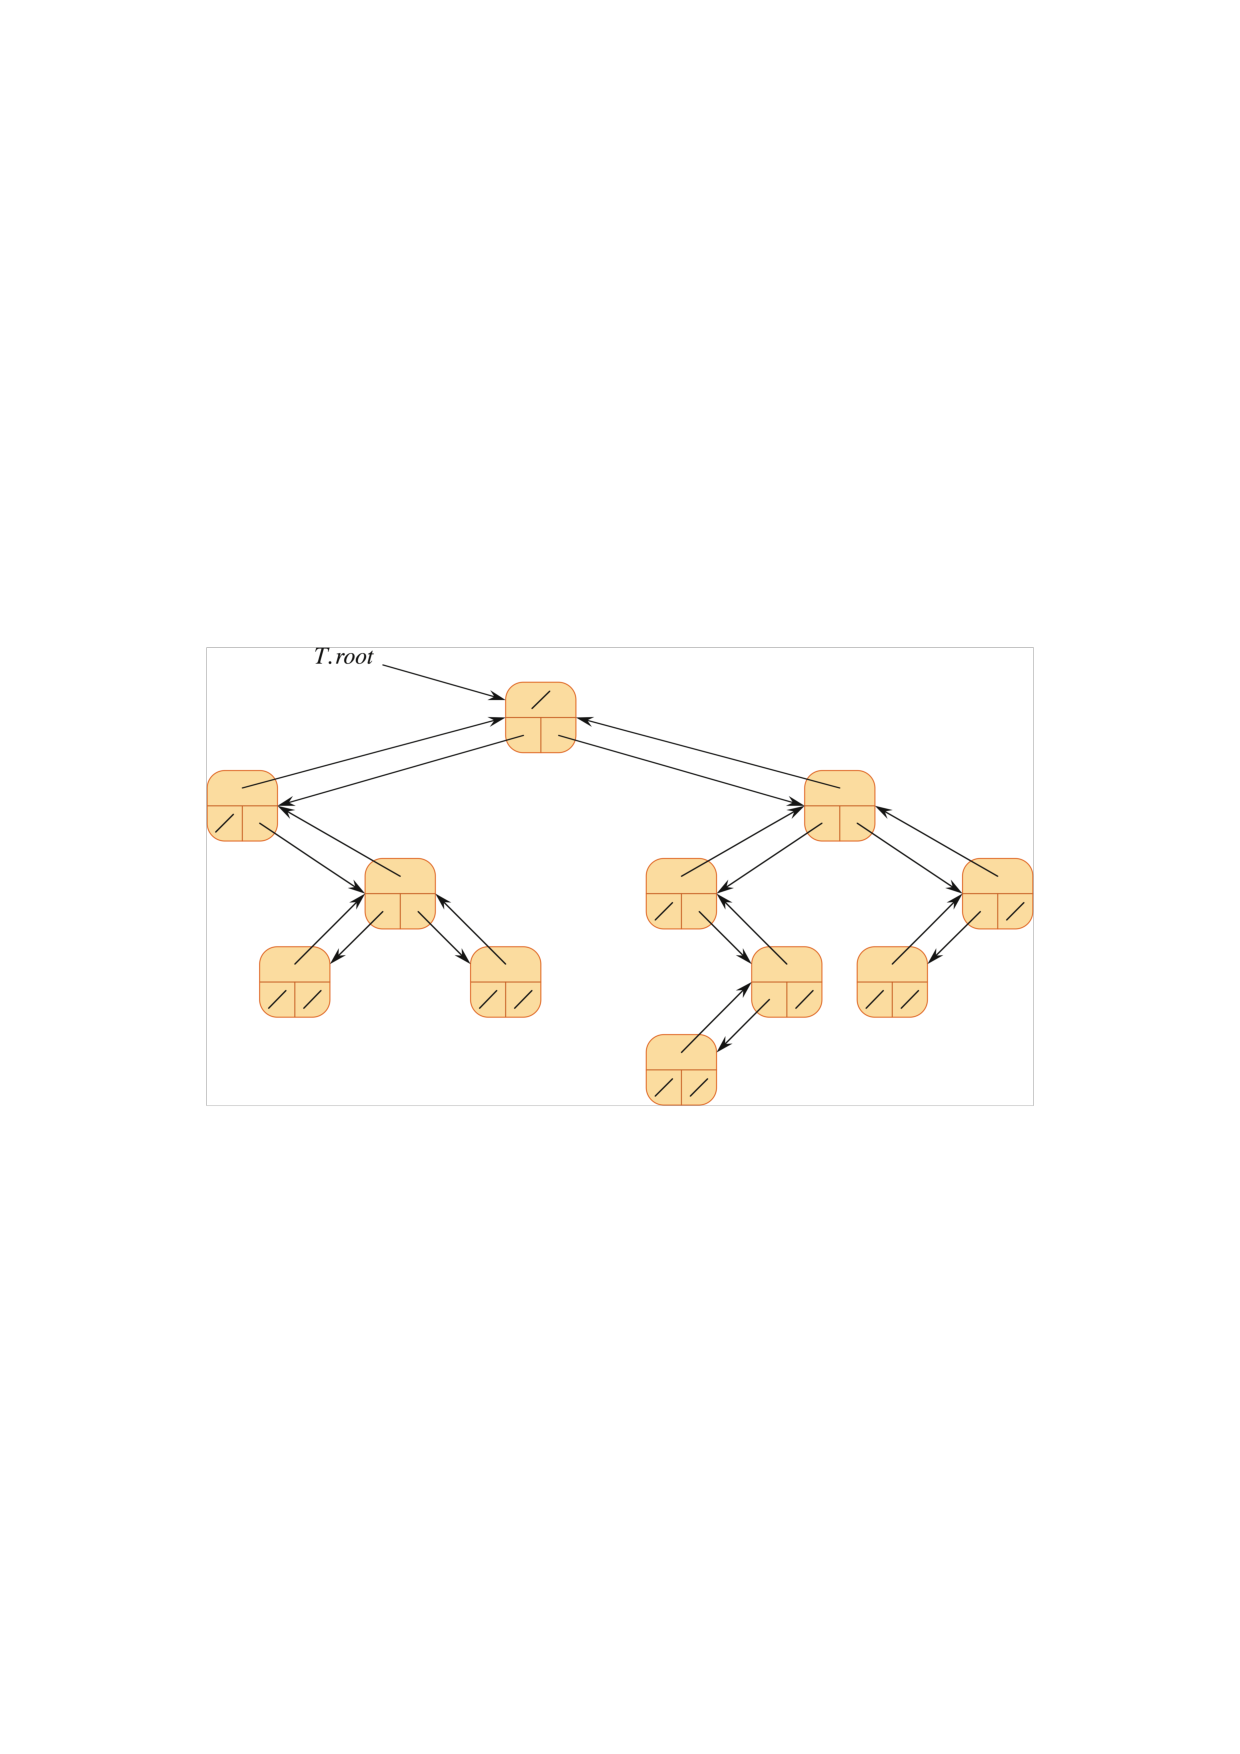
\includegraphics[width=\columnwidth]
			{fig/fig-TreeBinary}
		{\tiny
		\begin{tikzpicture}
			\tikzset{every leaf node/.style={font=\sffamily}}
			\Tree
			[.{parent}
				[.{node} 
					[.{root of LeftSubtree} ]
					[.{root of RightSubtree} ]
				]
			]
		\end{tikzpicture}		
		} % fsize
	\end{column} % ++++ A
	\end{columns} % <<<<
\end{frame}
% ~~~~~~~~~~~~~~~~~~~~~~~~~~~~~~~~~~~~~~ A




\subsection{MyNode}
% ~~~~~~~~~~~~~~~~~~~~~~~~~~~~~~~~~~~~~~ V
\begin{frame}[t]\frametitle{MyNode in Java}
	\vspace{-0.3cm}
	\begin{columns}[T] % >>>>
	\begin{column}{.5\linewidth} % ++++ V
		{\tiny 
		\begin{algorithm}[H]
			\SetKwData{Data}{\texttt{data}}
			\SetKwData{P}{\texttt{parent}}
			\SetKwData{L}{\texttt{left}}
			\SetKwData{R}{\texttt{right}}
			\Begin{
				\Data\\
				\P	\tcp*[f]{{\tiny reference to the parent}}\\
				\L	\tcp*[f]{{\tiny reference to the left child}}\\
				\R	\tcp*[f]{{\tiny reference to the right child}}\\
			    
				\caption{{\footnotesize Node for binary tree}}
			}
		\end{algorithm}
		} % \tiny

		\vspace{1cm}
		{\footnotesize 
			\hEmph{\texttt{MyNode}}  implements interface \hEmph{\texttt{NodeBinaryI}}.
		} % fsize
	\end{column} % ++++ A
	\begin{column}{.51\linewidth} % ++++ V
		{\tiny 
			\lstinputlisting[style=mystyle, language=Java]
				{input/input-java-NodeBinaryI.src}
		} % \tiny
		{\tiny 
			\lstinputlisting[style=mystyle, language=Java]
				{input/input-java-MyNode-Constructor.src}
		} % \tiny
	\end{column} % ++++ A
	\end{columns} % <<<<

\end{frame}
% ~~~~~~~~~~~~~~~~~~~~~~~~~~~~~~~~~~~~~~ A




\subsection{MyTree}
% ~~~~~~~~~~~~~~~~~~~~~~~~~~~~~~~~~~~~~~ V
\begin{frame}[t]\frametitle{MyTree in Java: Constructors}
	\vspace{-0.3cm}
	\begin{columns}[T] % >>>>
	\begin{column}{.5\linewidth} % ++++ V
		{\tiny 
			\lstinputlisting[style=mystyle, language=Java]
				{input/input-java-MyTree-Constructor.src}
		} % \tiny
	\end{column} % ++++ A
	\begin{column}{.51\linewidth} % ++++ V
		{\tiny 
			\lstinputlisting[style=mystyle, language=Java]
				{input/input-java-NodeBinaryI.src}
		} % \tiny
		{\tiny 
			\lstinputlisting[style=mystyle, language=Java]
				{input/input-java-MyNode-Constructor.src}
		} % \tiny
	\end{column} % ++++ A
	\end{columns} % <<<<

\end{frame}
% ~~~~~~~~~~~~~~~~~~~~~~~~~~~~~~~~~~~~~~ A




% ~~~~~~~~~~~~~~~~~~~~~~~~~~~~~~~~~~~~~~ V
\hSubsection{Implementation}{Navigation in Trees}
% ~~~~~~~~~~~~~~~~~~~~~~~~~~~~~~~~~~~~~~ A




% ~~~~~~~~~~~~~~~~~~~~~~~~~~~~~~~~~~~~~~ V
\begin{frame}[t]\frametitle{Navigation}
	\vspace{-0.3cm}
	\begin{columns}[T] % >>>>
	\begin{column}{.5\linewidth} % ++++ V
		\vspace{-0.3cm}
		{\tiny 
			\lstinputlisting[style=mystyle, language=Java]
				{input/input-java-MyTree-Navigation-traverse.src}
		} % \tiny
		{\tiny 
			\lstinputlisting[style=mystyle, language=Java]
				{input/input-java-LibTree-traverseInOrder.src}
		} % \tiny
	\end{column} % ++++ A
	\begin{column}{.51\linewidth} % ++++ V
		\vspace{-0.3cm}
		{\tiny 
			\lstinputlisting[style=mystyle, language=Java]
				{input/input-java-NodeBinaryI.src}
		} % \tiny
		{\tiny 
			\lstinputlisting[style=mystyle, language=Java]
				{input/input-java-MyNode-Navigation.src}
		} % \tiny
	\end{column} % ++++ A
	\end{columns} % <<<<

\end{frame}
% ~~~~~~~~~~~~~~~~~~~~~~~~~~~~~~~~~~~~~~ A



% ~~~~~~~~~~~~~~~~~~~~~~~~~~~~~~~~~~~~~~ V
\begin{frame}[t]\frametitle{Navigation: InOrder}
	\vspace{-0.3cm}
	\begin{columns}[T] % >>>>
	\begin{column}{.5\linewidth} % ++++ V
		\vspace{-0.3cm}
		{\tiny 
			\lstinputlisting[style=mystyle, language=Java]
				{input/input-java-MyTree-Navigation-traverse.src}
		} % \tiny
%		{\tiny 
%			\lstinputlisting[style=mystyle, language=Java]
%				{input/input-java-MyTree-Navigation-traverse-inorder.src}
%		} % \tiny
		{\tiny 
			\lstinputlisting[style=mystyle, language=Java]
				{input/input-java-LibTree-traverseInOrder.src}
		} % \tiny
	\end{column} % ++++ A
	\begin{column}{.52\linewidth} % ++++ V
		\vspace{-0.3cm}
		{\tiny 
			\begin{tikzpicture}
	\tikzset{every leaf node/.style={font=\sffamily}}
	\Tree
	[.$\times$
		[.$+$
			[.$8$ ]
			[.$7$	 ]
		]
		[.$-$
			[.$5$ ]
			[.$2$ ]
		]
	]
\end{tikzpicture}

		} % \tiny
		\vspace{-0.15cm}
		{\tiny 
			\lstinputlisting[style=mystyle, language=Java]
				{input/input-java-MyTree-Navigation-inorder-test.src}
		} % \tiny
		\hCodeOutputOnly{input/input-java-MyTree-Navigation-inorder-test}[3.8][2]
	\end{column} % ++++ A
	\end{columns} % <<<<

\end{frame}
% ~~~~~~~~~~~~~~~~~~~~~~~~~~~~~~~~~~~~~~ A



% ~~~~~~~~~~~~~~~~~~~~~~~~~~~~~~~~~~~~~~ V
\begin{frame}[t]\frametitle{Navigation: InOrder, PreOrder, PostOrder}
	\vspace{-0.3cm}
	\begin{columns}[T] % >>>>
	\begin{column}{.5\linewidth} % ++++ V
		\vspace{-0.3cm}
		{\tiny 
			\lstinputlisting[style=mystyle, language=Java]
				{input/input-java-MyTree-Navigation-traverse.src}
		} % \tiny
%		{\tiny 
%			\lstinputlisting[style=mystyle, language=Java]
%				{input/input-java-MyTree-Navigation-traverse-inorder.src}
%		} % \tiny
		{\tiny 
			\lstinputlisting[style=mystyle, language=Java]
				{input/input-java-LibTree-traverseInOrder.src}
		} % \tiny
	\end{column} % ++++ A
	\begin{column}{.52\linewidth} % ++++ V
		\vspace{-0.3cm}
%		{\tiny 
%			\begin{tikzpicture}
	\tikzset{every leaf node/.style={font=\sffamily}}
	\Tree
	[.$\times$
		[.$+$
			[.$8$ ]
			[.$7$	 ]
		]
		[.$-$
			[.$5$ ]
			[.$2$ ]
		]
	]
\end{tikzpicture}

%		} % \tiny
		{\tiny 
			\lstinputlisting[style=mystyle, language=Java]
				{input/input-java-LibTree-traverse-all.src}
		} % \tiny
%		\vspace{-0.3cm}
%		\hCodeOutputOnly{input/input-java-MyTree-Navigation-inorder-test}[10][0.5]
	\end{column} % ++++ A
	\end{columns} % <<<<

\end{frame}
% ~~~~~~~~~~~~~~~~~~~~~~~~~~~~~~~~~~~~~~ A




% ~~~~~~~~~~~~~~~~~~~~~~~~~~~~~~~~~~~~~~ V
\hSubsection{Implementation}{Other Recursive Methods}
% ~~~~~~~~~~~~~~~~~~~~~~~~~~~~~~~~~~~~~~ A




% ~~~~~~~~~~~~~~~~~~~~~~~~~~~~~~~~~~~~~~ V
\begin{frame}[t]\frametitle{Plot}
	\vspace{-0.3cm}
	\begin{columns}[T] % >>>>
	\begin{column}{.5\linewidth} % ++++ V
		{\tiny 
			\lstinputlisting[style=mystyle, language=Java]
				{input/input-java-MyTree-plot.src}
		} % \tiny
		\vspace{-0.1cm}
		{\tiny 
			\lstinputlisting[style=mystyle, language=Java]
				{input/input-java-LibTree-plot.src}
		} % \tiny
	\end{column} % ++++ A
	\begin{column}{.51\linewidth} % ++++ V
		{\tiny 
			\lstinputlisting[style=mystyle, language=Java]
				{input/input-java-NodeBinaryI.src}
		} % fsize
		{\scriptsize
		\begin{example}
			\begin{tikzpicture}
	\tikzset{every leaf node/.style={font=\sffamily}}
	\Tree
	[.$1$
		[.$2$
			[.$4$ ]
			[.$5$	 ]
		]
		[.$3$
			[.$6$ ]
%			[.$\hGround$ ]
			[.$.$ ]
		]
	]
\end{tikzpicture}

		\end{example}
		} % fsize
		
		\hCodeOutputOnly{input/input-java-LibTree-plot}[3][-1.5]
	\end{column} % ++++ A
	\end{columns} % <<<<
\end{frame}
% ~~~~~~~~~~~~~~~~~~~~~~~~~~~~~~~~~~~~~~ A




% ~~~~~~~~~~~~~~~~~~~~~~~~~~~~~~~~~~~~~~ V
\begin{frame}[t]\frametitle{Height}
	\vspace{-0.3cm}
	\begin{columns}[T] % >>>>
	\begin{column}{.5\linewidth} % ++++ V
		{\tiny 
			\lstinputlisting[style=mystyle, language=Java]
				{input/input-java-MyTree-height.src}
		} % \tiny
		\vspace{-0.1cm}
		{\tiny 
			\lstinputlisting[style=mystyle, language=Java]
				{input/input-java-LibTree-height.src}
		} % \tiny
	\end{column} % ++++ A
	\begin{column}{.51\linewidth} % ++++ V
		{\tiny 
			\lstinputlisting[style=mystyle, language=Java]
				{input/input-java-NodeBinaryI.src}
		} % fsize
		{\scriptsize
		\begin{example}
			\begin{tikzpicture}
	\tikzset{every leaf node/.style={font=\sffamily}}
	\Tree
	[.$1$
		[.$2$
			[.$4$ ]
			[.$5$	 ]
		]
		[.$3$
			[.$6$ ]
%			[.$\hGround$ ]
			[.$.$ ]
		]
	]
\end{tikzpicture}

			
			Call 
			{\tiny \texttt{MyBinaryTree\_Test.height\_constructBT\_S\_1\_6()}}
			{\scriptsize \texttt{MyBinaryTree\_Test.height\_constructBT\_S\_1\_6()}}
		\end{example}
		} % fsize
		
		\hCodeOutputOnly{input/input-java-LibTree-height}[4][-1]
	\end{column} % ++++ A
	\end{columns} % <<<<
\end{frame}
% ~~~~~~~~~~~~~~~~~~~~~~~~~~~~~~~~~~~~~~ A


% ~~~~~~~~~~~~~~~~~~~~~~~~~~~~~~~~~~~~~~ V References bib
\begin{frame}[t,allowframebreaks]\frametitle{References}
	\setbeamertemplate{bibliography item}[text] % sets numbers in references
%	\bibliographystyle{abbrv}
%	\bibliographystyle{apalike}
%	\bibliographystyle{ieeetr}
	\bibliographystyle{IEEEtran}
	%
	\tiny\bibliography{../hbcommon/bingol-DataStructures} % bib file

	
\end{frame}
% ~~~~~~~~~~~~~~~~~~~~~~~~~~~~~~~~~~~~~~ A

% ~~~~~~~~~~~~~~~~~~~~~~~~~~~~~~~~~~~~~~~ 
\end{document}
